%%%%%%%%%%%%%%%%%%%%%%%%%%%%%%%%%%%%%%%%%%%%%%%%%%%%%%%%%%%%%%%%%%%%%%%%%%%%%%%%
%2345678901234567890123456789012345678901234567890123456789012345678901234567890
%        1         2         3         4         5         6         7         8

\documentclass[letterpaper, 10 pt, conference]{ieeeconf}  % Comment this line out if you need a4paper

%\documentclass[a4paper, 10pt, conference]{ieeeconf}      % Use this line for a4 paper

\IEEEoverridecommandlockouts                              % This command is only needed if 
                                                          % you want to use the \thanks command

\overrideIEEEmargins                                      % Needed to meet printer requirements.

%In case you encounter the following error:
%Error 1010 The PDF file may be corrupt (unable to open PDF file) OR
%Error 1000 An error occurred while parsing a contents stream. Unable to analyze the PDF file.
%This is a known problem with pdfLaTeX conversion filter. The file cannot be opened with acrobat reader
%Please use one of the alternatives below to circumvent this error by uncommenting one or the other
%\pdfobjcompresslevel=0
%\pdfminorversion=4

% See the \addtolength command later in the file to balance the column lengths
% on the last page of the document

% The following packages can be found on http:\\www.ctan.org
\usepackage{graphicx} % for pdf, bitmapped graphics files
%\usepackage{epsfig} % for postscript graphics files
%\usepackage{mathptmx} % assumes new font selection scheme installed
%\usepackage{times} % assumes new font selection scheme installed
\usepackage{amsmath} % assumes amsmath package installed
\usepackage{amssymb}  % assumes amsmath package installed
\usepackage[linesnumbered, lined, boxed, commentsnumbered, ruled, vlined]{algorithm2e} % package for writing pseudo code

\usepackage[dvipsnames]{xcolor}

\title{\LARGE \bf
Correct-by-synthesis reinforcement learning with temporal logic constraints*
}


\author{Karan Muvvala$^{1}$ % <-this % stops a space
\thanks{*This work was originally done by Wen et al.\cite{c1}}% <-this % stops a space
\thanks{$^{1}$Karan Muvvala is a graduate student associated with Department of Mechanical Engineering,
        University of Colorado Boulder, Boulder, CO 80309, USA
        {\tt\small karan.muvvala@colorado.edu}}%
% \thanks{$^{2}$Bernard D. Researcheris with the Department of Electrical Engineering, Wright State University,
%         Dayton, OH 45435, USA
%       {\tt\small b.d.researcher@ieee.org}}%
}


\begin{document}



\maketitle
\thispagestyle{empty}
\pagestyle{empty}


%%%%%%%%%%%%%%%%%%%%%%%%%%%%%%%%%%%%%%%%%%%%%%%%%%%%%%%%%%%%%%%%%%%%%%%%%%%%%%%%
\begin{abstract}

Autonomous systems are gradually ubiquitous. Beyond simply demonstrating these systems, it is becoming increasingly important to provide formal guarantees that they will behave safely and reliably while also completing the task at hand. The interaction between the robot and the environment can be modelled as a two-player game. Using tools developed by the Formal methods community we can compute permissive strategies that satisfy certain temporal constraints that can be specified within the LTL framework. We then consider the problem of synthesis of optimal strategy that performs the given task optimally with respect to some a priori unknown performance criterion encoded as rewards. Thus, we decouple the problem into subproblems. \textcolor{black}{First, we extract a (maximally) permissive strategy for the system, which encodes multiple (possibly all) ways in which the system can react to an adversarial environment.}  Then, we compute an optimal strategy within this envelope of valid strategies. Thus, we can guarantee both qualitative(encoded as the winning condition) and quantitative (optimal reactive controller) performance for a system operating in an unknown environment. 


\end{abstract}


%%%%%%%%%%%%%%%%%%%%%%%%%%%%%%%%%%%%%%%%%%%%%%%%%%%%%%%%%%%%%%%%%%%%%%%%%%%%%%%%
\section{INTRODUCTION}

%The goal of this project is to reproduce the %results of the work done by Wen et al. in\cite{c1}.% 
\textcolor{black} {The goal of the paper is to synthesize optimal reactive strategies for systems} with respect to the underlying task with some unknown performance criterion  assuming an adversarial environment while also satisfying temporal specifications. A strategy dictates which action(s) to take given the current situation the robot is in. Formally, it's a mapping from a given state to an action and can be non-deterministic. With temporal constraints on the strategies we guarantee certain behavior traits which encode safety guarantees e.g do not collide with the obstacles. Temporal constraints also put restrictions on the sequence of actions that can be taken e.g visit region 1 and then visit region 2 while always avoiding region 3. These constraints can be defined for both finite horizon and infinite horizon tasks thus providing qualitative guarantees on the strategies synthesized. Thus, general requirements on system behavior such as safety concerns and task specific rules may be known and expressed as temporal specification.\\

\textcolor{black}{On the other hand, quantitative performance criteria can help encode more subtle considerations} which can be tailor made to the scenario and task at hand. With the growing use of autonomous systems, we need to provide safety guarantees on these systems for them to be accepted by the society - for an autonomous vehicle a safety constraint could be \textcolor{black} {e.g always drive in the correct lane, never jump red light and eventually reach the destination}. While tools like \cite{c2} and \cite{c3} developed by the Formal methods community can be leveraged to devise strategies that can guarantee task completion while also satisfying these constraints.We then can integrate them with tools developed by the learning community to compute optimal strategies (with respect to some underlying unknown performance criterion) within the envelope of acceptable strategies synthesized before, thus taking into account quantitative  behaviors. \\

\textcolor{black}{The two main topics relevant to this work are reactive synthesis with temporal logic specification and reinforcement learning with respect to unknown performance criterion}.  The approach of decoupling the problem into two subproblems - 1)extracting permissive strategy\cite{c4}, which encodes multiple(possible all) ways in which the system can interact to the environment and 2)learning the unknown performance criterion as a reward function using reinforcement learning algorithms is a completely novel approach. Up until the time of the publication of\cite{c1}, the above problem as a whole was unconsidered, even though several aspects concerning the qualitative behavior and the quantitative behavior have been well studied before independently.

\section{Related Work}

Recently robots have achieved incredible capability to perform fairly complex tasks. But, these performances are limited to static environments \cite{c4}-\cite{c8}. To make these robots robust to the environment they are operating in, they should be able to react to the changes thus guaranteeing task completion despite interference i.e they need to perform the task reactively - take actions based on the observation of the changes from the previous time step in the world\cite{c9}-\cite{c10}. There have also been studies that looked into synthesizing optimal strategies while satisfying temporal specifications but only consider deterministic environments with known transition distribution\cite{c11}-\cite{c12}.\\

\textcolor{black}{Learning the a priori unknown performance criterion} can be gained through experience from interactions in the given environment. Many reinforcement learning methods\cite{c13} have focused on this aspect such as Q-learning, SARSA and Monte Carlo methods. However, these processes cannot guarantee the satisfaction of the given temporal constraints \textcolor{black} {while also maximizing the expected rewards} at the same time. \\

Since the publication of the original paper, recent works have focused on using using similar approaches such as learning the unknown cost function while satisfying certain safety constraints\cite{c14} and synthesizing a shield\cite{c15} which continuously monitors the actions taken by the learner and correct them if and only if the chosen action causes a violation of the specification. Both these approaches try to integrate safety by first computing a set of strategies that behave as per the specification (i.e only allow certain transitions) and then learn in this new constrained state-space.

\section{Preliminaries}

I now introduce some preliminaries relevant to the project.

\subsection{Two-player Games}

Games are commonly used to model the interaction between two rational agents operating in the same state space. Two-player games model the interaction between two players - often the environment is modeled as a player that behaves stochastically and the system (the controlled agent/ system robot) as another player. Formally, it can be defined as follows:\\

\textcolor{black}{ \textbf{Definition 1.} \textit{A two-player game, or simply a game is defined as a tuple $G = (S, S_s, s_e, I,A_c, A_{uc}, T, W)$, where $S$ is a finite set of states; \{$S_s, S_e$\} is a partition of $S$, i.e, $S = S_s \cup S_e, S_s \cap S_e = \emptyset; I \subseteq S$ is a set of initial states; $A_c$ is a finite set of controlled actions of the system;$A_{uc}$ is a finite set uncontrolled actions for the environment and $A_{uc} \cap A_c = \emptyset;\: T : S \times \{A_c \cup A_{uc}\} \rightarrow 2^S$ is a transition function; $W$ is the winning condition defined later.}}\\

The environment agent and the system agent can only choose an action at state $S_e$ and $S_s$. $A_c$ is the set of actions associated with the system agent and $A_{uc}$ is the set of actions associated with the environment agent. Here we assume $G$ to be deterministic i.e the transition function $T$ satisfies $|T(s, a)| \leq 1$.\textcolor{black}{ Without loss of generality all states are reachable from $I \in G$.}

\subsection{Linear Temporal Logic}

In this paper we consider that specifications are given as formulas($\phi$) of a particular type of logic, called Linear Temporal Logic(LTL). These formulas can efficiently capture an array of properties, including safety(nothing bad will ever happen) and liveness properties(something good will eventually happen) and more complex combinations of Boolean and temporal statements. \\

In LTL we can reason about temporal formulas that are constructed from a set of observations, Boolean operators, and temporal operators. The set of Boolean formulas are ($\top$ (true), $\neg$ (negation), $\wedge$ (conjunction)) and temporal operator \bigcirc(next), $\cup$ (until) and the derived temporal operators like $\square$(always), $\lozenge$(eventually) and any (nested) combination of them, like $\square \lozenge$ (always-eventually) and $\lozenge \square$ (eventually-always). Formally, given a set of atomic propositions we define the syntax of LTL formulas as follows:\\

\textbf{Definition 2.} \textit{(LTL Syntax) A (propositional) Linear Temporal Logic (LTL) formula $\phi$ over a given set of propositions $p$ is recursively defined as}

\begin{equation}
\phi = p \; \arrowvert\;  \phi_1 \wedge \phi_2\;  \arrowvert\; \neg \phi\; \arrowvert\; \bigcirc \phi\; \arrowvert\; \phi_1 \cup \phi_2
\end{equation}

where $p \in AP$ is an atomic proposition. An atomic proposition is a Boolean variable (or propositional variable). $AP$ is usually a finite set and in our case $AP = O$ (set of observation).

To obtain the full expressivity of propositional logic, additional operators such as $\vee$ (disjunction), $\rightarrow$(implies) and $\leftrightarrow$ (if and only if) can be combined with any two formulas as follows: 

\begin{itemize}
    \item $\phi_1 \vee \phi_2 = \neg(\neg \phi_1 \wedge \phi_2)$
    \item $\phi_1 \rightarrow \phi_2 = \neg \phi_1 \vee \phi_2 $
    \item $\phi_1 \leftrightarrow \phi_2 = (\phi_1 \rightarrow \phi_2) \wedge (\phi_2 \rightarrow \phi_1)$
\end{itemize}\\

In addition, the temporal operators $\lozenge$("eventually") and $\square$("always") are defined as follows:

\begin{itemize}
    \item $\lozenge \phi = \top \cup \phi$
    \item $\square \phi = \neg \lozenge \neg \phi$
\end{itemize}\\

LTL formulas are interpreted over infinite words made of observations from $AP$, i.e over $(2^{AP})^w$(set of infinite sequence of set of propositions). Formally, the LTL semantics are defined as follows:\\

\textbf{Definition 3.}\textit{(LTL Semantics) The satisfaction of formula $\phi$ over a set of Atomic propositions($AP$) at position $K \in \mathbb{N_+}$ by word $w_o =w_o(1)w_o(2)w_o(3)... \in AP^w $, denoted by $w_o(k) \models \phi$, is defined recursively as follows:}
\begin{itemize}
     \item
    $w_o(k) \models p \; \text{for some}\; p \in AP   \; \text{if}\; w_o(k) = p,$ 
    \item 
    $w_o(k) \models \neg \phi\; \text{if} \; w_o(k) \not\models \phi$
    \item
    $w_o(k) \models \phi_1 \wedge \phi_2\; \text{if}\; w_o(k) \models \phi_1\; \text{and}\; w_o(k) \models \phi_2$
    \item
    $w_o(k) \models \bigcirc \phi\; \text{if}\; w_o(k+1) \models \phi$\
    \item
    $w_o(k) \models \phi_1\: \cup\: \phi_2\: \text{if there exists}\: j \geq k\: \text{such that}\: w_o(j) \models \phi_2,\text{and, for all}\; k \leq i < j,\; \text{we have}\; w_o(i) \models \phi_1 $
\end{itemize}

where $\models$ is interpreted as "satisfies"\\

\textcolor{black}{Let $AP$ be a set of atomic propositions, then we can define a labelling function $L : S \rightarrow 2^{AP}$ such that each states $s \in S$ is mapped to the set of atomic propositions that hold \textit{True} at state $s$. A word is an infinite sequence of labels $L(\pi) = L(s_0)L(s_1)L(s_2)...$ where $\pi = s_0, s_1, s_2...$ is a run on $G$. We say that a run $\pi \models \phi$ if and only if $L(\pi) \models \phi$.}\\

For our construction we define a winning condition $W = (L, \phi)$ a tuple of labelling function and an formula $\phi$ defined within the LTL framework, and \textcolor{black}{ a run $\pi$ of $G$ is winning for the system if and only if $\pi \models \phi$.} \\

For our particular case, we use Slugs toolbox\cite{c2} which is built around the General Reactivity(1)(GR(1)) framework. The specifications in this fragment of LTL are of the form Assumptions $\rightarrow$ Guarantees. Formally, the specification is written as follows:

\begin{equation}
    \phi^a_i + \phi^a_s + \phi^a_l \longrightarrow  \phi^g_i + \phi^g_s + \phi^g_l
\end{equation}

Here, $\phi_i^a$ is the initialization assumption, $\phi_s^a$ is the safety assumption, $\phi_l^a$ is the liveness assumption. Assumptions, the first set of formulas, are used to state what we know about the behavior of the environment in which the synthesized system is intended to operate in. Guarantees, the set of formulas after the implication ($\rightarrow$), are certain behavior properties that the synthesized system needs to satisfy if the environment behaves as expected.  For e.g safety assumption could be - avoid collision with the environment robot, and liveness assumption could be - visit cell $N$ and then $N^2 - 1$ in $G$(where $N$ is the size of the environment e.g 3). We can define safety and liveness $assumptions$ on the environment robot while enforcing a different set of safety and liveness $guarantees$ on the system robot . 
 
\subsection{Control Strategies}

\textcolor{black} {Given the game $G$, we would like to synthesize a control strategy such that the runs of $G$ satisfy the specification.}  A (deterministic) stationary/memoryless strategy for the system is a mapping $\mu : S_s \rightarrow A_c$ where $A_c$ is the set of actions available at that given state $s \in S_s$.\\

A run $\pi = s_0s_1s_2…$ is induced by a strategy $\phi$ for the system if for any $i \in \mathbb{N}$ such that $s_i \in S_s,\; s_{i+1} = T(s_i, \mu(s_i))$. \textcolor{black}{ Let $R^{\mu}(s)$ be the set of runs of $G$ induced by a strategy $\mu$} for the system initialised from $s \in I$. $|R^{\mu}(s)| > 1$ when the strategies for the environment are not unique, even if $\mu$ is deterministic.\\

We say a strategy $\mu$ is said to win from a given state $s \in S$ if all the runs $\pi$ induced by it $R^{\mu}(s)$ are winning for the system. A strategy is called a winning strategy if it wins from all the states $s \in I$ of $G$.  Hence,\textcolor{black} {a formula $\phi$ is $realizable$ for $G$ if there exists a winning strategy for the system with $W = (L, \phi)$. }

\subsection{Reward Function}

Now that we can guarantee qualitative performance through permissive strategies defined over specification within the LTL framework with temporal constraints, we can consider quantitative evaluations modeled as reward functions which we ideally want to maximize by choosing the most optimal strategy that also satisfies temporal constraints.\\  

\textcolor{black} {To evaluate system strategies} we either map each state or a state-action pair to an non-negative value called as the state value $v$ and action value $q$ respectively using an \textcolor{black} {instantaneous reward function $R : S_s \times (A_c \cup A_{uc}) \rightarrow \mathbb{R}^{+} \cup \{0\}$.}\\

As runs over the game $G$ can be infinite, we introduce the discounted sum of rewards $(J^{G}_R)$ function  to compute a fixed value for an infinite sequence of states. Formally, it can expressed as follows:

\textcolor{black}{
\begin{equation}
    J^{G}_R = \sum_{k=0}^{\infty}  \gamma^k R_{k+1}
\end{equation}}

Here $\gamma$ also known as the discount factor is a value  between $0 \leq \gamma < 1$ and $R_{k+1}$ is the instantaneous reward obtained at the $(k + 1)$ time step.  Now we defined the reward function \textcolor{black} {$\bar{J}^{G}_R : P \times S_s \rightarrow R^{+} \cup \{0\}$ to evaluate each strategy for the system, where $P$ is the set of system strategies. Usually $|R^{\mu}(s)| > 1$ as the uncontrolled environment has more than one strategies, and thus the definition of $\bar{J}_R^G(\mu, s)$ is not unique given $J_R^G(\pi)$ for all the runs in $R^{\mu}(s)$. One commonly used choice for $\bar{J}_R^G$ is the expectation of $J_R^G(\pi)$ over all the runs in $R^{\mu}(s)$ with some given distribution for the environment strategy, i.e $\mathbb{E}_{\pi \in R^{\mu}(s)}[J_R^G(\pi)]$. The distribution is usually estimated from interaction experience with the environment. Another common way is to define $\bar{J}_R^G$ as the minimal possible reward acquired when the system strategy is $\mu$, i.e,}

\textcolor{black}{
\begin{equation}
    \bar{J}^G_R(\mu, s) = \inf_{\pi \in R^{\mu}(s)} J_R^G(\pi) ,
\end{equation}
}


which is the reward function in our case.

\section{Problem Formulation}

Now that we have formally defined games, strategies and the reward function we can formulate the problem formally.

\subsection{Problem Definition}

\textcolor{black} {\textbf{Problem 1.}\textit{ A two-player deterministic game $G = (S, S_s, S_e, I, A_c, A_uc, T, W)$ is given where $W = (L, \phi)$ is the winning condition and $\phi$ is realizable for $G$. Find a memoryless or finite memory winning strategy $\mu$ for the system such that $\bar{J}^{G}_R(\mu, s)$ is maximized for all states $s \in I$, where $\bar{J}^{G}_R$ is the instantaneous reward as defined by equation 4.}}\\

We can decouple our approach in two sub-problems. We first extract a non-deterministic winning strategy $\mu_p$ called a permissive strategy\cite{c4} , which guarantees that $R^{\mu} \subseteq R^{\mu_p}(s)$, for all memoryless winning strategies $\mu$ and $s \in I$.  Then we restrict to the transitions allowed by $\mu_p$,\textcolor{black} {apply reinforcement learning methods to explore the a priori unknown instantaneous reward function $R$ and compute an optimal strategy} over all the strategies of the new game obtained in the first stage.

\section{Strategy Synthesis}

In this section, I formally define what permissive strategies are and their significance in safety only specifications. Then I briefly introduce the concept of Markov Games and the reinforcement learning algorithm implemented. Finally, I lay out the algorithm used to compute the optimal strategy for a system robot operating in an adversarial environment.

\begin{figure*}[t]
    \centering
    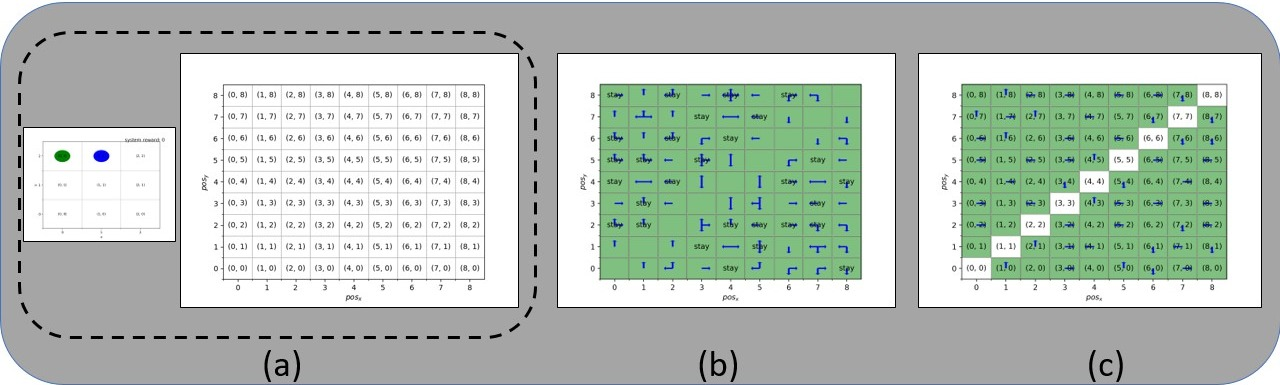
\includegraphics[width=\textwidth]{images/trimmed_algo_vis_hq.jpg}
    \caption{Visualization of Algorithm 1. The figure on the left (a) represents the construction of the game $G$ for a 3 x 3 grid world($N = 3$). The system robot(green pebble) can control only the $pos_x$ variable and the environment robot(blue pebble) can control only the $pos_y$ variable respectively.Note:(a) represents only the system robot's state space(cells) (b)We then compute a (maximally)permissive strategy $\mu_p^{max}$ for a specification $\phi$ from Slugs. The arrows indicate action(s) that the system robot(system strategy) can take from each cell. Left and right arrow mean -1 and +1 value respectively of the $pox_x$ value which is the variable controlled by the system player. An up and down arrow mean +3 ans -3(width of the original grid world ($N$)) value of the $pos_x$ variable. (c)This plot represents the learned optimal policy by the system robot to achieve the given task for Example 1.}
\label{fig:my_label}
\end{figure*}

\subsection{Permissive Strategy}

As described above, the interaction between the system robot and the environment(modeled as a robot that can not be controlled by the system robot) can be interpreted as a two-player game.  A permissive strategy is a strategy that tries to capture all the behaviours of all the memoryless strategies. Formally, a permissive strategy can be defined as\\

% \footnote{}

\textcolor{black} {\textbf{Definition 4.}\textit{ Given a two-player game G, a non-deterministic strategy $\mu$ for the system is called permissive if (i) it is winning for the system and (ii) includes all memoryless winning strategies for the system. A permissive strategy is called maximally permissive if it includes all winning strategies for the system.}}\\

All two-player games have permissive strategies. For games with finite states, there are only finitely many memoryless winning strategies. Extracting maximally permissive strategies is desirable as they allow all possible behaviors of all the memoryless strategies winning on $G$ for specification $\phi$.\\

\textcolor{black} {\textbf{Proposition 1.}\cite{c4}\textit{ All games $G$ with winning conditions $W = (L, \phi)$ in which $\phi$ is a safety formula must have memoryless or finite-memory maximally permissive strategies.}}\\

I use the software tool slugs to extract (maximally) permissive strategies $\mu_p^{max}$ as I only consider safety properties in my specifications $\phi$. These specifications can be extended to include liveness properties but has been skipped as it is beyond the scope of this project. Under proposition 1, slugs synthesizes a maximally permissive strategy.\\

Thus, by extracting permissive strategies guaranteeing qualitative behavior, we can then focus on quantitative properties by optimizing the performance of these strategies which are known to satisfy the temporal constraints. We then apply $\mu_p^{max}$ to the game $G$ and update the transition function $T$ to remove all the transitions that are not allowed by the strategies $\mu_p^{max}$. We then construct $\hat{G}$ and try to learn the $\hat{\mu}^*$ that maximizes the reward function for all states $s \in \hat{I}$. 


\subsection{Reinforcement Learning}

Now that we have constructed $\hat{G}$ \textcolor{black} {whose runs are all guaranteed to be correct with respect to the underlying LTL specification}, we can now learn an optimal strategy with respect to an a priori unknown reward function $R$. The objective of the reinforcement learning algorithm is to maximize $\bar{J}^{\hat{G}}_R$ for the game $\hat{G}$.\\

As described in  section II.D, we make use of a discounted sum of rewards function to evaluate the rewards obtained by a run and particularly focus on the \textcolor{black}{ minimal (worst-case) possible reward for each system strategy} which can be considered as a tight lower bound of the reward obtained by executing strategy $\hat{\mu}$ for any strategy played by the environment robot. Assuming the environment plays adversarially, the game can be considered as a zero-sum game.  The reward gained by the system and the environment are additive inverse of each other.\\ 

I then apply generalized Q-learning for alternating Markov games\cite{c16} with an $\epsilon$-greedy strategy for choosing action. There are theoretical proofs that the greedy strategy learned, which always chooses an action with the best learned Q value, converges to an optimal strategy for a system interacting with an adversary.

\subsection{Algorithm}

Now that we have formally defined $G$, $\mu_p$(permissive strategies) and the reward function $R$ used, we couple these as mentioned in Algorithm 1. Fig 1. shows a visualization of the implementation on a 3 x 3 grid world ($N$ = 3). \\ 

We first construct the grid world in which both the system robot and the environment robot operate in. Then we construct the game $G$ with $N^2 - 1$ cells for each robot for a given specification $\phi$ in GR(1) format and compute the maximally permissive strategy $\mu_p^{max}$ and then apply this to the game $G$ to remove all undesirable behaviors (transitions) to construct $\hat{G}$. The cells with no actions represent invalid states because the robots are in collision. With the new game $\hat{G}$ we then apply Q-learning to compute the optimal strategy $\hat{\mu}$ as shown in Fig 1.c for the task in Example 1. The Pseudo-algorithm for this as process is elaborated in Algorithm 1.\\

% \textcolor{red}
\begin{algorithm}
    \SetAlgoLined
    \SetKwData{Left}{Left}\SetKwData{This}{This}\SetKwData{Up}{Up}
    \SetKwInOut{Input}{Input}\SetKwInOut{Output}{Output}
    \Input{\textcolor{black} {A game $G = (S, S_s, S_e, I, A_c, A_{uc}, T, W)$ with $W = (L, \phi)$ in which $\phi$ is a realizable formula for $G$, a reward function $J_R^G$ and $\bar{J}_R^G$(as in (4)) with respect to an unknown instantaneous reward function $R$}}
    \Output{\textcolor{black}{A winning strategy $\mu$ for the system that maximizes $\bar{J}_R^G(\mu, s)$ for all $s \in I$}}
    
    \Begin{
    \textcolor{black}{
    Compute a (maximally) perimssive strategy $\mu_p$}
    
    \textcolor{black}{
    Apply $\mu_p$ to $G$ and modify $G$ into a new game $\hat{G} = (\hat{S, \hat{S_s}, \hat{S_e}, \hat{I}, A_c, A_{uc}, \hat{T}, \hat{W}})$, where $\hat{W} = (L, True)$.}
    
    \textcolor{black}{
    Compute $\hat{\mu}_p^*$ that maximizes $\hat{J}_{R(\mu, s)}^{\hat{G}}$ for all $s \in \hat{I}$ with some reinforcement algorithm (I use tabular Q-learning)}
    
    \textcolor{black}{
    Map $\hat{\mu}_p^*$ in $\hat{G}$ back to $\mu^*$ in $G$
    }
    }
\caption{Pseudo-algorithm for solving Problem 1.}

\end{algorithm}

% \textcolor{black}
As we are also considering reactive safety properties, we can compute maximally permissive strategy. Thus the strategy $\mu_p$ includes all the winning strategies and is a winning strategy itself.  

\section{Examples}

As a proof of concept we consider a finite horizon robot motion planning problem in a grid world of different sizes in Example 1. I then expand this to a grid world with obstacles in it for a given task in LTL for Example 2.  In both these cases we can compute a maximally permissive strategy $\mu_p^{max}$ for a given specification $\phi$ with only safety properties.\\

\textbf{Example 1.} Let two robots, the system robot and the environment robot move in a $N \times N$ square grid world in a turn based situation, i.e. first the system robot takes an action and only after executing this action does the environment robot take an action and execute it. Initially both the robots are in different locations and the task for the system robot is to always be in a diagonally opposite position to the environment robot while avoiding collision with the environment robot. One key assumption is that the grid world is fully observable meaning each robot has information relevant to the position of the other robot at any given instance of time.\\

\textcolor{black}{The problem can be formulated as a game $G = (S, S_s, S_e, I, A_c, A_{uc}, T, W)$ with $W = (L, \phi)$. Let $Pos = \{0,...,N^2 - 1\}$ be the set of cells in the map. Then $S = Pos \times Pos \times \{0, 1\},\; S_s = Pos \times Pos \times \{1\},\; S_e = Pos \times Pos \times \{0\}.\; I = \{(x, y, 1)\: \vert\: x, y, \in Pos, x \not= y\}$. $A_c = \{up_s, down_s, left_s, right_s, stay_s\},\: A_{uc} = \{up_e, down_e, left_e, right_e \}$. The Transition function $T$ guarantees that $A_c$ and $A_{uc}$ only change the first and the second component of a state respectively. The set of Atomic proposition $AP = (\bigcup_{i=0}^{N^2 -1} x_i) \cup  (\bigcup_{j=0}^{N^2 -1} y_j) \cup \{t_o, t_1\}$. The labeling function is $L(s)= \{x_i, y_j, t_k\}$ if $s = (i, j, k) \in S.$ The system specification can be written as }
\textcolor{black}{
\begin{equation}
    \phi_0 = \bigwedge_{i=0}^{N^2 -1}(\neg x_i \vee \neg y_i) \wedge \square \bigwedge_{i=0}^{N^2 -1} (x_i \rightarrow \neg y_i)    
\end{equation}
}
The specification $\phi_0$ can be interpreted as follows; $\phi_i$ the initial specification says that both the robots should not start in the same cell. The safety property $\phi_s$ mentions that the \textit{system robot} should not take a transition that leads to a collision. The same is not true for the environment robot and thus the strategy $\mu_p$ for the system robot and the environment robot won't be same.\\ 

According to Proposition 1. we can compute $\mu_p^{max}$ (maximally permissive strategy) and then construct $\hat{G}$. Following Algorithm 1. we compute the optimal strategy $\mu^*$. The reward is as defined in (4) and the value of discount factor $\gamma$ is set to 0.9. \textcolor{black} {$R$ here is set to encourage the system robot to reach positions diagonal to the environment robot’s position as often as possible. From a state $s \in S_s$.\: $R(s, a) = +1$ if the two robots are diagonal to each other at $T(s, a)$, otherwise $R(s, a) = 0$ .} The results for the cases when $N = 3,4,5,6,7$ are shown in Table I.

\begin{table}[h]
\caption{Results for Example 1.}
\label{table_example}
\begin{center}
\begin{tabular}{|c|c|c|c|c|c|}
\hline
N & $t_e(s)$ & $t_l(s)$ & Iterations (x $10^3$) & $\hat{S}$ & $\hat{S_s}$ \\
\hline
3 & 0.027 & 159.13 & 41 & 162 & 72\\
\hline
4 & 0.047 & 625.23 & 137 & 512 & 240\\
\hline
5 & 0.251 & 5236.11 & 1000 & 1250 & 600\\
\hline
6 & 0.321 & 13704.94 & 2000 & 2592 & 1260\\
\hline
7 & 0.401 & 8066.6 & 1000 & 4802 & 1640\\
\hline
\end{tabular}
\end{center}
\end{table}

Time $t_e$ is the time spent in computing the maximally permissive strategy $\mu_p^{max}$.\; $t_l$ is the time spent learning the optimal strategy $\hat{\mu}^*$ for the game $\hat{G}$.  For $N = 5,6\: \text{and}\: 7$ the algorithm reached the maximum number of iterations before converging. For this project I created my own environment and wrote a naive Q-learning implementation. I believe that by building my environment in OpenAI gym\cite{c17} and implementing OpenAI baseline algorithms, which are a collection of high-quality implementations of reinforcement learning algorithms, I can speed up the learning process and work with grid worlds with $N > 20$. 

Now, I illustrate the optimality of the learned greedy policy for $N = 6$ as shown in Fig 2. Let $\hat{\mu}$ be the greedy strategy of the system learned by the Q-learning algorithm against an adversarial environment. If from a state $\hat{s} \in \hat{S}_s$ the system robot can only reach a diagonal position with respect to the position of the environment in at least $k \in \mathbb{N}$ steps, \textcolor{black}{ $\bar{J}_{R}^{\hat{G}}(\hat{\mu}', s)$ is upper bounded by $\sum_{l=k}^{\infty} \gamma^l.1 = \frac{1}{1-\gamma}\gamma^k$ for any system strategy $\hat{\mu}^*$ is an optimal strategy for the system against an adversarial environment, we have} 
\textcolor{black}{
\begin{equation}
    \bar{J}_R^{\hat{G}}(\hat{\mu}', s) \leq \bar{J}_R^{\hat{G}}(\hat{\mu}*, s) \leq 
    \frac{1}{1-\gamma}\gamma^k
\end{equation}
}
In the $6 \times 6$ case, the system can always reach a diagonal position in 5 steps. Fig 2. shows that the state value $V$ converges to the values $10,9, 8.1,7.29,6.561,5.905$ which coincide with $\frac{1}{1-\gamma}\gamma^k$ when $k = 0,1,2,3,4,5$ and $\gamma = 0.9$.\\ 

Thus by the inequality in (6), $\bar{J}_R^{\hat{G}}(\hat{\mu}, \hat{s})$ also coincide with $\bar{J}_R^{\hat{G}}(\hat{\mu}^*, \hat{s})$, \textcolor{black} {indicating that $\hat{\mu}$ itself is an optimal strategy of the system, as predicted by Algorithm 1}. \\

\begin{figure}[t]
    \centering
    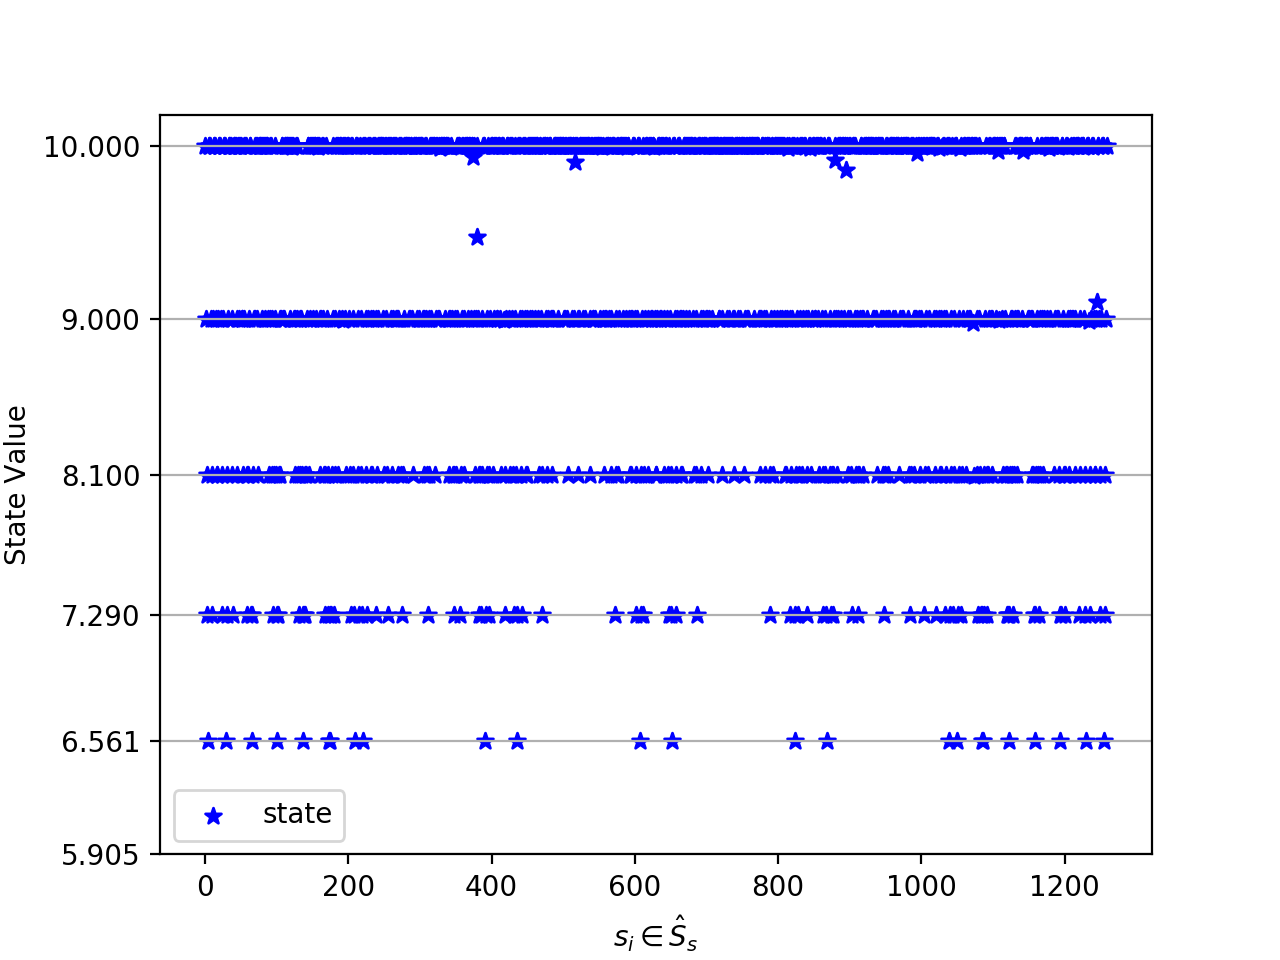
\includegraphics[width=0.5\textwidth]{images/State Value_N_6.png}
    \caption{Results for Example 1 for $N = 6$. $\bar{J}_R^{\hat{G}}(\hat{\mu}, \hat{s})$ for all $\hat{s} \in \hat{S}_s$ and the learned greedy strategy $\hat{\mu}$}
\label{fig:state value N_6}
\end{figure}

\begin{figure}[b]
    \centering
    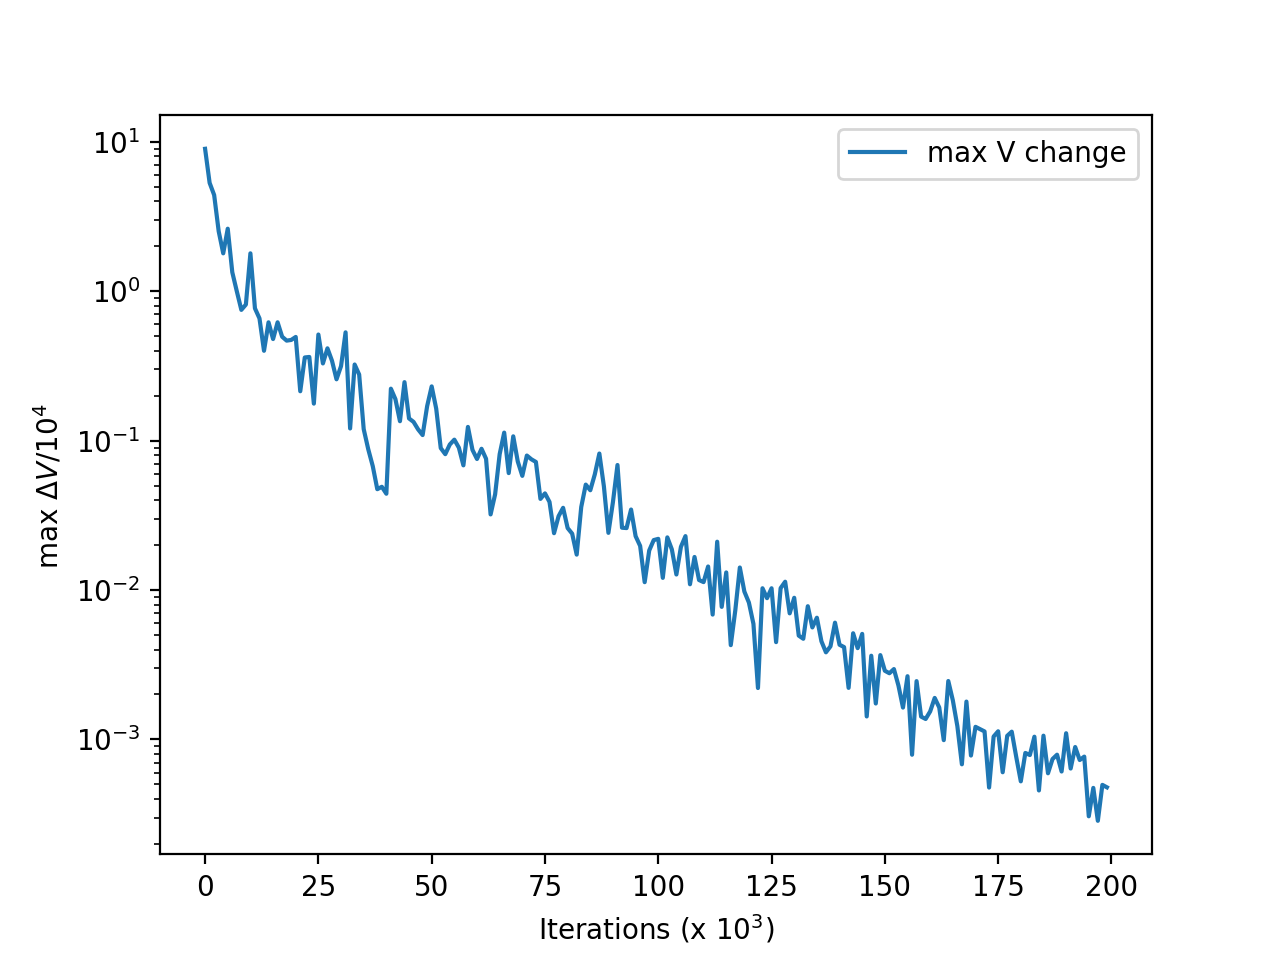
\includegraphics[width=0.5\textwidth]{images/max del_V_per_10k_N_6.png}
    \caption{The Logarithm of the maximal change in $V$ in every $10^4$ iterations}
\label{fig:max del(v) N 6}
\end{figure}

\textbf{Example 2.} In this example, I include 2 static obstacles that the robots need to avoid while ensuring completion of the given task. For the sake of simplicity everything from Example 1. remains the same except for the inclusion of obstacles in the environment. The original grid world is as shown in Fig 4.  and the learned policy for N = 7 is shown in Fig 5. \\

In Fig 5. the white blocks represent the states in which the system robot and the environment robot are in collision. The gray cells represent the cells occupied by the obstacles. High resolution pictures and other supplementary material can be found at https://github.com/MuvvalaKaran/CoRL in the README and under the directories src/two\_player\_game/plot and src/figures\_and\_gifs.


\begin{figure}[t]
    \centering
    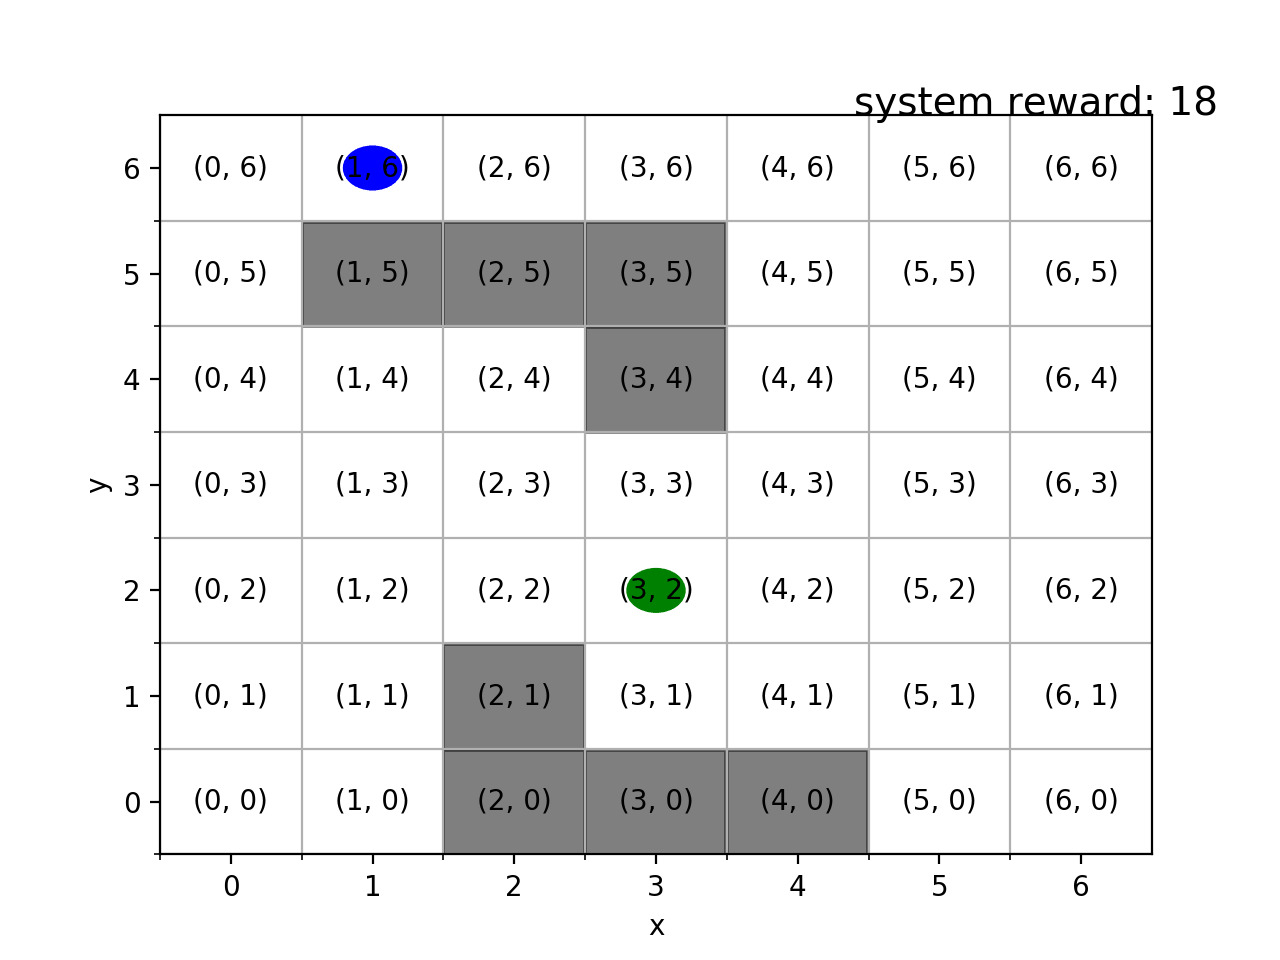
\includegraphics[width=0.5\textwidth]{images/N_7_grid_world.jpg}
    \caption{The grid world for $N= 7$ with two static obstacles}
\label{fig:N 7 grid world}
\end{figure}

\begin{figure}[t]
    \centering
    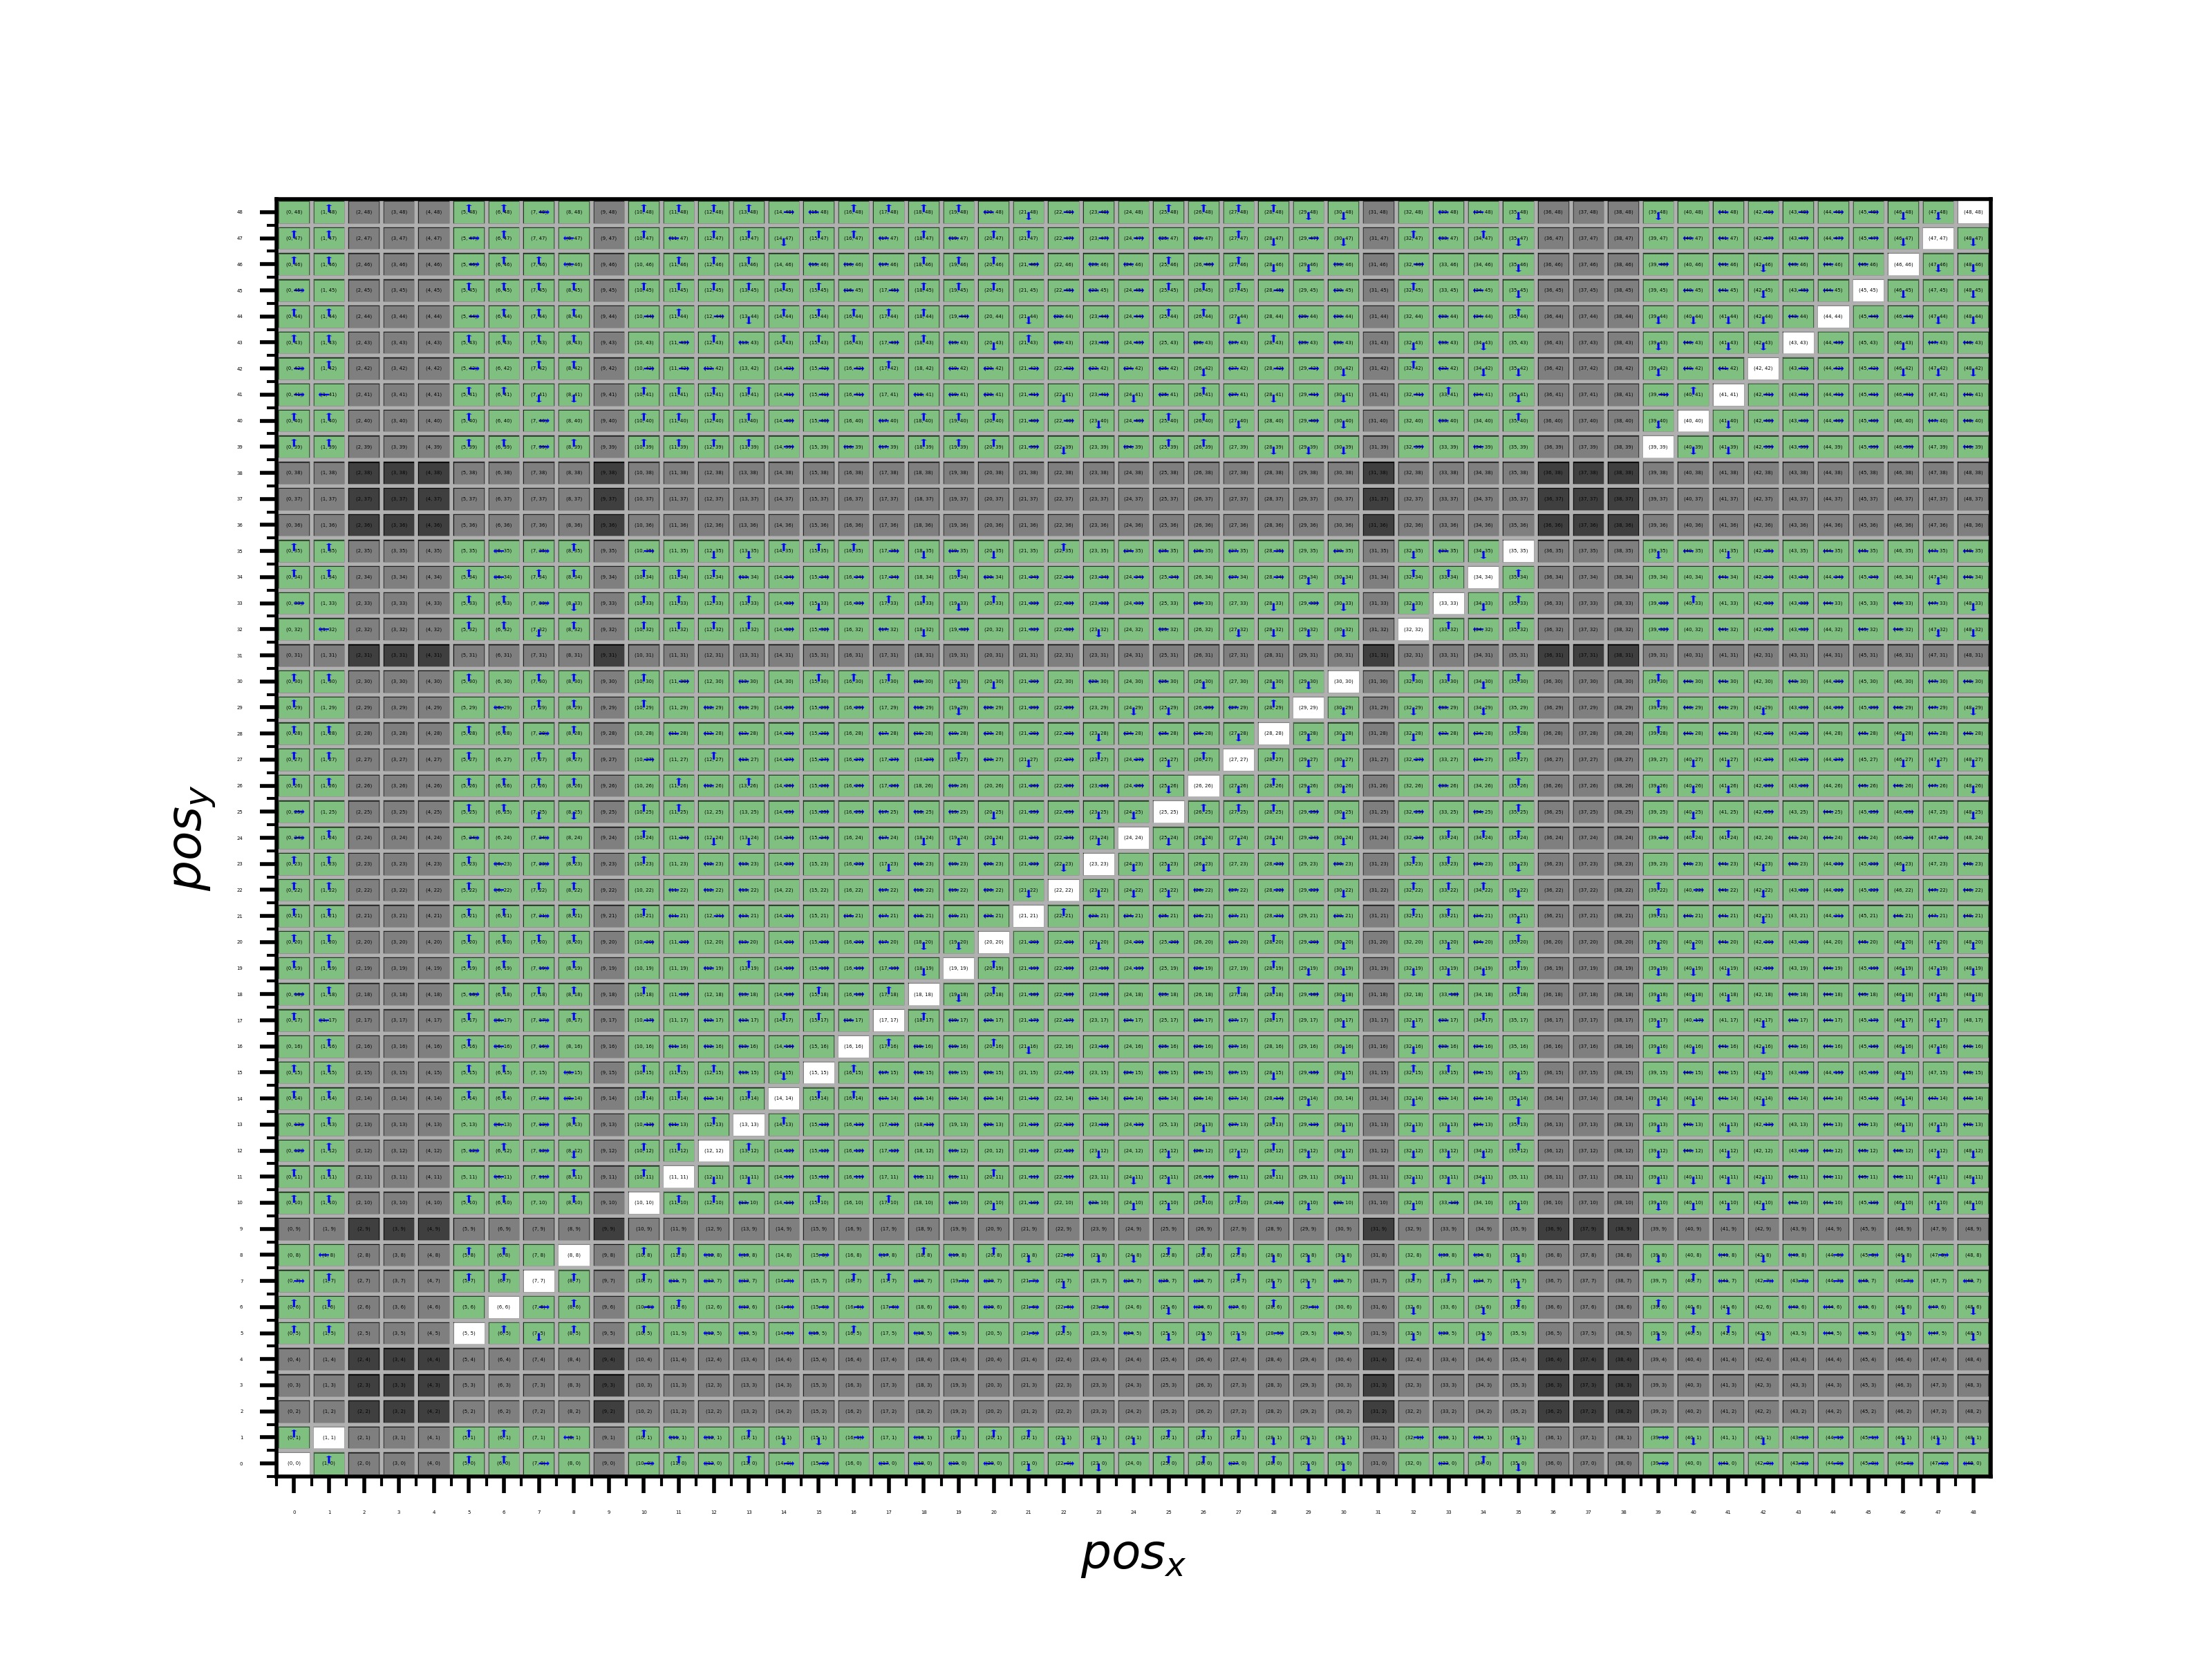
\includegraphics[width=0.5\textwidth]{images/Policy for G_hat_N_7_N_7.png}
\caption{The learned policy for $N = 7$. Gray boxes are cells occupied by the obstacles.}
\label{fig:policy N 7}
\end{figure}


\section{Future work}

We can expand our specifications $\phi$ to include liveness properties as well.  For example, we can say that the system robot should \textcolor{black} {visit the upper left corner (cell $N^2 - N$) and the lower right corner (cell $N-1$) infinitely often, provided that the environment robot visits the lower left corner (cell $0$) and the upper right corner (cell $N^2 -1$) infinitely often}. In such cases the specification can be written as
\textcolor{black}{
\begin{equation}
    \phi_1 = \phi\: \bigwedge\: ((\square\lozenge x_0 \vee \square\lozenge x_{N^2 - 1}) \rightarrow (\square\lozenge y_{N - 1} \vee \square\lozenge y_{N^2 - N}))
\end{equation}
}
In this situation we cannot compute a maximally permissive strategy and hence the expected true value $\bar{J}_R^{\hat{G}}(\hat{\mu}, \hat{s})$ should be almost the same as $\bar{J}_R^{\hat{G}}(\hat{\mu}^*, \hat{s})$, as the system robot is allowed to follow $\hat{\mu}^*$ for as many finite moves as desired. But $\bar{J}_R^{\hat{G}}(\hat{\mu}, \hat{s})$ is smaller, indicating that the \textcolor{black} {system strategy is sub-optimal due to the loss of some winning strategies by the permissive strategy} $\mu_p$

\section{Conclusion}

We can compute optimal reactive controllers for robots operating in dynamic environments under temporal logic constraints defined within GR(1); a fragment of LTL. The decoupled approach allows us to apply the best of both the communities and the results are discussed in section VI.

\section{Acknowledgment}

I would like to thank all the authors of the original paper for clarifying all my queries related to implementation and helping me throughout the course project with their valuable advice and insights. 

\begin{thebibliography}{99}
\bibitem{c1}Wen, Min, Rüdiger Ehlers, and Ufuk Topcu. "Correct-by-synthesis reinforcement learning with temporal logic constraints." 2015 IEEE/RSJ International Conference on Intelligent Robots and Systems (IROS). IEEE, 2015.
\bibitem{c2}R. Ehlers, V. Raman, and C. Finucane. Slugs GR(1) synthes izer, 2013– 2014.  Available  at https://github.com/LTLMoP/slugs
\bibitem{c3} Bloem, R., Jobstmann, B., Piterman, N., Pnueli, A., Sa'ar, Y.:  Synthesis of reac-tive(1) designs.  J. Comput. Syst. Sci.78 (3) (2012) 911-938
\bibitem{c4}  J.  Bernet,  D.  Janin,  and  I.  Walukiewicz.   Permissive  stra tegies:  from parity  games  to  safety  games. RAIRO-Theoretical  Informatics  and Applications ,  36(03):261–275,  2002.
\bibitem{c5}L. P. Kaelbling and T. Lozano-P ́ erez, “Hierarchical task and motion planning in the now,” in International Conference on Robotics and Automation .  IEEE, 2011
\bibitem{c6}S. Srivastava, E. Fang, L. Riano, R. Chitnis, S. Russell, and P. Abbeel, “Combined task and motion planning through an extensible planner-independent interface layer,” in International Conference on Robotics and Automation .  IEEE, 2014
\bibitem{c7}K. He, M. Lahijanian, L. E. Kavraki, and M. Y. Vardi, “Towards manip-ulation planning with temporal logic specifications,” in International Conference on Robotics and Automation .  IEEE, May 2015
\bibitem{c8}N. T. Dantam, Z. K. Kingston, S. Chaudhuri, and L. E. Kavraki, “Incremental task and motion planning: a constraint-based approach,” inRobotics: Science and Systems , 2016
\bibitem{c9}He, Keliang, et al. "Reactive synthesis for finite tasks under resource constraints." 2017 IEEE/RSJ International Conference on Intelligent Robots and Systems (IROS). IEEE, 2017.
\bibitem{c10}A. Pnueli and R. Rosner. On the synthesis of an asynchron ous reactive module.  InAutomata, Languages  and Programming , pages 652–671. Springer,  1989
\bibitem{c11} X.  C.  Ding,  S.  L.  Smith,  C.  Belta,  and  D.  Rus.    Optimal  contr ol of  markov  decision  processes  with  linear  temporal  logic  con straints. IEEE Transactions  on Automatic Control ,  59(5):1244–1257,  2014
\bibitem{c12}C.  J.  Watkins  and  P.  Dayan.   Q-learning.Machine  Learning ,  8(3-4):279–292,  1992
\bibitem{c13} R. S. Sutton and A. G. Barto.Introduction to Reinforcement Learning . MIT Press, 1998.
\bibitem{c14}Junges, Sebastian, et al. "Safety-constrained reinforcement learning for MDPs." International Conference on Tools and Algorithms for the Construction and Analysis of Systems. Springer, Berlin, Heidelberg, 2016.
\bibitem{c15}Jansen, Nils, et al. "Shielded decision-making in MDPs." arXiv preprint arXiv:1807.06096 (2018).
\bibitem{c16} M.  L.  Littman  and  C.  Szepesv ́ari.     A  generalized  reinfor cement-learning  model:  Convergence  and  applications.    In Proceedings  of Conference  on Machine Learning ,  pages 310–318,  1996
\bibitem{c17}Brockman, Greg, et al. "Openai gym." arXiv preprint arXiv:1606.01540 (2016).

\end{thebibliography}

\end{document}